\documentclass{article}
\usepackage{graphicx} % Required for inserting images

\title{Labwork 3 Advanced Programming for HPC}
\author{Ta Quang Hieu - M22ICT002}
\date{October 2023}

\begin{document}
	
	\maketitle
	
	\section{The problem}
	Labwork 5: Map
	
	\section{Binarization}
	Figure ~\ref{fig:python} the image that I used for this problem:
	
	\begin{figure}
		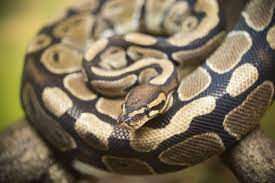
\includegraphics[width=\linewidth]{python.jpg}
		\caption{A python in rgb.}
		\label{fig:python}
	\end{figure}
	
	This is the mapping function that I used to achieve Binarization.
	
	\begin{verbatim}
		@cuda.jit(nopython=True)
		def binarization(x):
		threshold = 20
		if x < threshold:
		return 0
		return 1
	\end{verbatim}
	
	Figure ~\ref{fig:binarization} is the result produced from the mapping function and the kernel:
	
	\begin{figure}
		
\includegraphics[width=\linewidth]{binarization.png}
		\caption{Binarization result.}
		\label{fig:binarization}
	\end{figure}
	
	As we can observe in Figure ~\ref{fig:binarization}, when applying binarization, my output image is just a black one.
	
	\section{Brightness control}
	Figure ~\ref{fig:python} the image that I used for this problem:
	
	\begin{figure}
		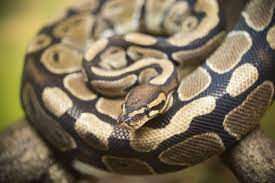
\includegraphics[width=\linewidth]{python.jpg}
		\caption{A python in rgb.}
		\label{fig:python}
	\end{figure}
	
	This is the mapping function that I used to achieve Brightness control.
	
	\begin{verbatim}
		@cuda.jit(nopython=True)
		def brightness(x, amount):
		if x + amount > 255:
		return 255
		elif x + amount < 0:
		return 0
		return x + amount
	\end{verbatim}
	
	Figure ~\ref{fig:brightness_control} is the result produced from the mapping function and the kernel that increase the brightness by 50 for each pixel:
	
	\begin{figure}
		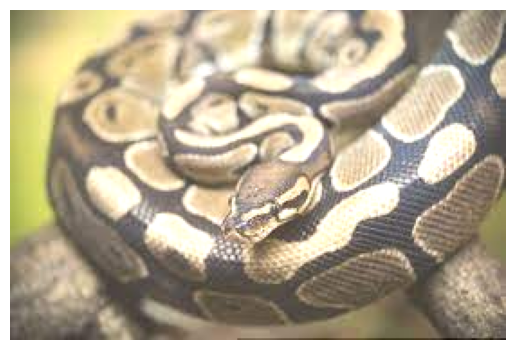
\includegraphics[width=\linewidth]{brightness_control.png}
		\caption{Brightness control result.}
		\label{fig:brightness_control}
	\end{figure}
	
	\section{Blending image}
	Figure ~\ref{fig:python} is the first image that I used for this problem:
	
	\begin{figure}
		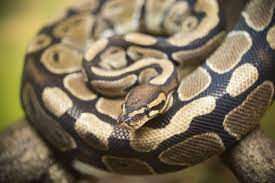
\includegraphics[width=\linewidth]{python.jpg}
		\caption{A python in rgb.}
		\label{fig:python}
	\end{figure}
	
	Figure ~\ref{fig:beautiful} is the second image that I used for this problem:
	
	\begin{figure}
		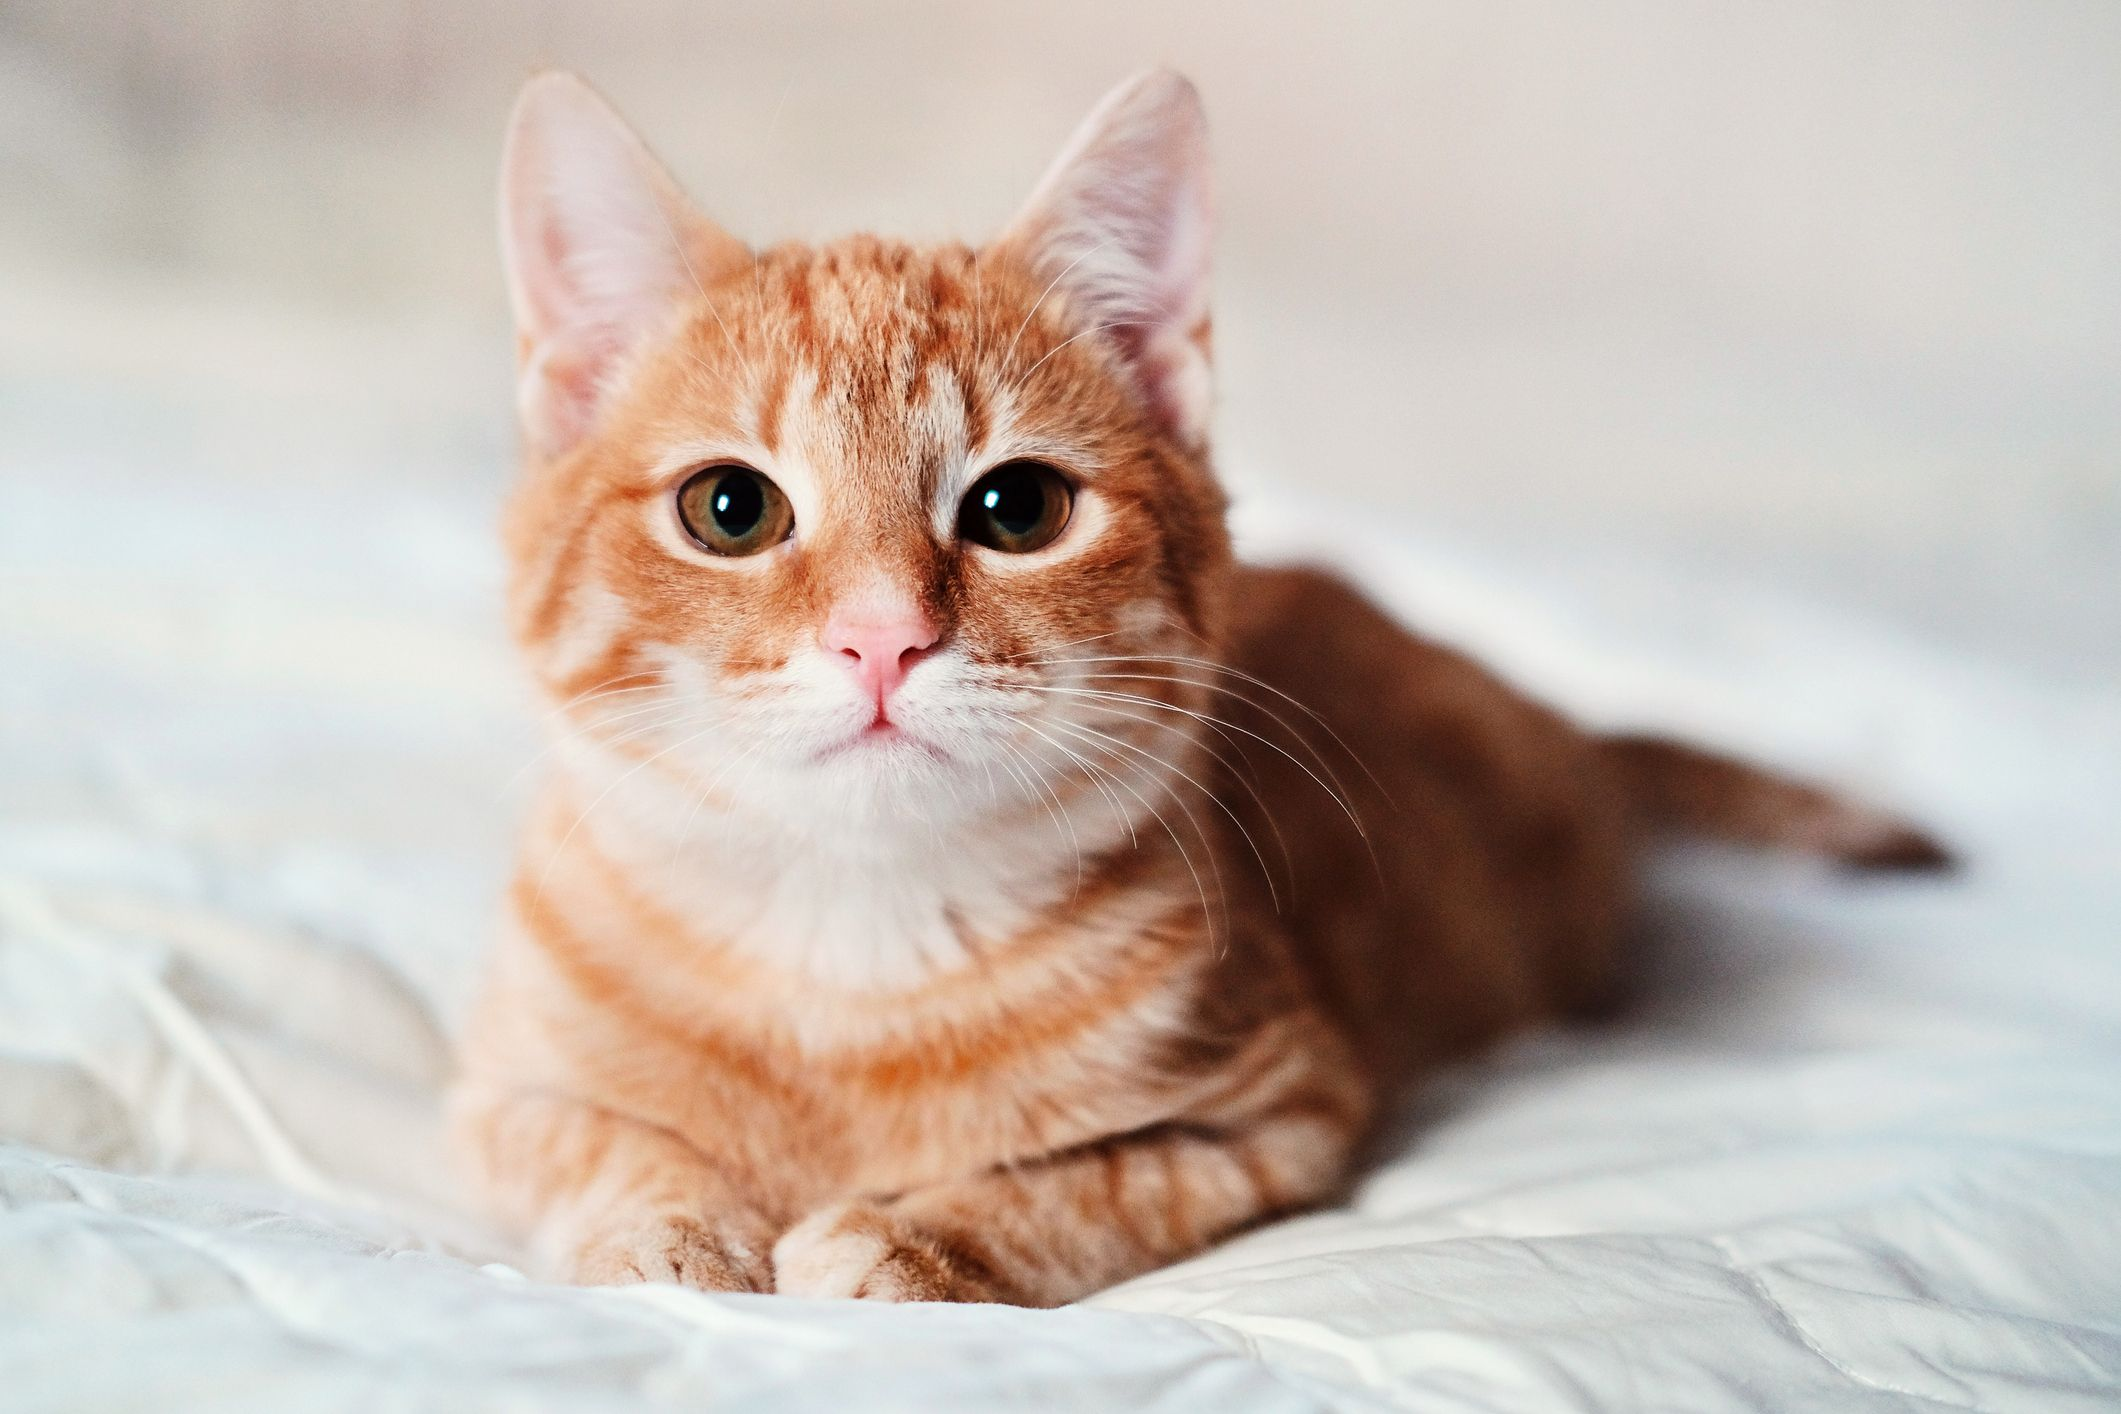
\includegraphics[width=\linewidth]{beautiful.jpg}
		\caption{A beautiful in rgb.}
		\label{fig:beautiful}
	\end{figure}
	
	This is the mapping function that I used to achieve Brightness control.
	
	\begin{verbatim}
		@cuda.jit(nopython=True)
		def blending(x, y):
		return np.uint8(0.2*x + 0.8*y)
	\end{verbatim}
	
	Figure ~\ref{fig:blending} is the result produced from the mapping function and the kernel that increase the brightness by 50 for each pixel:
	
	\begin{figure}
		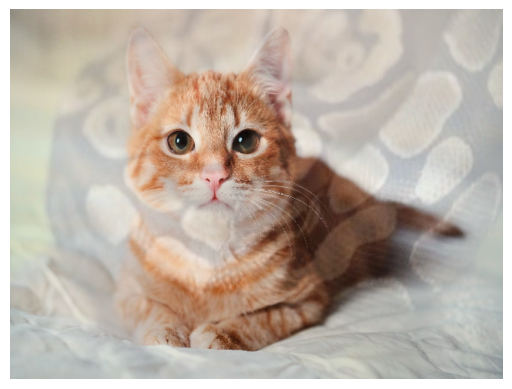
\includegraphics[width=\linewidth]{blending.png}
		\caption{Blending result.}
		\label{fig:blending}
	\end{figure}
	
	
\end{document}
